%
% fig-wege.tex
%
% (c) 2025 Prof Dr Andreas Müller
%
\begin{figure}
\centering
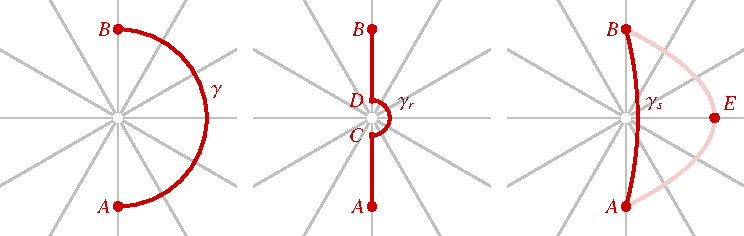
\includegraphics{chapters/030-kurvenintegral/images/wege.pdf}
\caption{Verschiedene Wege zur Berechnung des Integrals der 1-Form
$r\,d\varphi$.
Die Wege, die nahe am Nullpunkt vorbeigehen, ergeben nur sehr kleine
Werte für das Integral, während der Kreisbogen $\gamma$ des
Einheitskreises den Wert $\pi$ ergibt.
\label{buch:kurvenintegral:differential:fig:wege}}
\end{figure}
